%\documentclass[slides]{beamer} %switch "slides" to "handout" for printing out
\documentclass[handout]{beamer}

%packages
%\usepackage{latexsym}
\usepackage{graphicx}
\usepackage{color}
\usepackage{amsmath}
\usepackage{dsfont}
\usepackage{placeins}
\usepackage{amssymb}
\usepackage{wasysym}
\usepackage{abstract}
\usepackage{hyperref}
\usepackage{etoolbox}
\usepackage{datetime}
\usepackage{xcolor}
\usepackage{alphalph}
\settimeformat{ampmtime}

%\usepackage{pstricks,pst-node,pst-tree}

%\usepackage{algpseudocode}
%\usepackage{amsthm}
%\usepackage{hyperref}
%\usepackage{mathrsfs}
%\usepackage{amsfonts}
%\usepackage{bbding}
%\usepackage{listings}
%\usepackage{appendix}
\usepackage[margin=1in]{geometry}
%\geometry{papersize={8.5in,11in},total={6.5in,9in}}
%\usepackage{cancel}
%\usepackage{algorithmic, algorithm}

\makeatletter
\def\maxwidth{ %
  \ifdim\Gin@nat@width>\linewidth
    \linewidth
  \else
    \Gin@nat@width
  \fi
}
\makeatother

\definecolor{fgcolor}{rgb}{0.345, 0.345, 0.345}
\newcommand{\hlnum}[1]{\textcolor[rgb]{0.686,0.059,0.569}{#1}}%
\newcommand{\hlstr}[1]{\textcolor[rgb]{0.192,0.494,0.8}{#1}}%
\newcommand{\hlcom}[1]{\textcolor[rgb]{0.678,0.584,0.686}{\textit{#1}}}%
\newcommand{\hlopt}[1]{\textcolor[rgb]{0,0,0}{#1}}%
\newcommand{\hlstd}[1]{\textcolor[rgb]{0.345,0.345,0.345}{#1}}%
\newcommand{\hlkwa}[1]{\textcolor[rgb]{0.161,0.373,0.58}{\textbf{#1}}}%
\newcommand{\hlkwb}[1]{\textcolor[rgb]{0.69,0.353,0.396}{#1}}%
\newcommand{\hlkwc}[1]{\textcolor[rgb]{0.333,0.667,0.333}{#1}}%
\newcommand{\hlkwd}[1]{\textcolor[rgb]{0.737,0.353,0.396}{\textbf{#1}}}%

\usepackage{framed}
\makeatletter
\newenvironment{kframe}{%
 \def\at@end@of@kframe{}%
 \ifinner\ifhmode%
  \def\at@end@of@kframe{\end{minipage}}%
  \begin{minipage}{\columnwidth}%
 \fi\fi%
 \def\FrameCommand##1{\hskip\@totalleftmargin \hskip-\fboxsep
 \colorbox{shadecolor}{##1}\hskip-\fboxsep
     % There is no \\@totalrightmargin, so:
     \hskip-\linewidth \hskip-\@totalleftmargin \hskip\columnwidth}%
 \MakeFramed {\advance\hsize-\width
   \@totalleftmargin\z@ \linewidth\hsize
   \@setminipage}}%
 {\par\unskip\endMakeFramed%
 \at@end@of@kframe}
\makeatother

\definecolor{shadecolor}{rgb}{.77, .77, .77}
\definecolor{messagecolor}{rgb}{0, 0, 0}
\definecolor{warningcolor}{rgb}{1, 0, 1}
\definecolor{errorcolor}{rgb}{1, 0, 0}
\newenvironment{knitrout}{}{} % an empty environment to be redefined in TeX

\usepackage{alltt}
\usepackage[T1]{fontenc}

\newcommand{\qu}[1]{``#1''}
\newcounter{probnum}
\setcounter{probnum}{1}

%create definition to allow local margin changes
\def\changemargin#1#2{\list{}{\rightmargin#2\leftmargin#1}\item[]}
\let\endchangemargin=\endlist 

%allow equations to span multiple pages
\allowdisplaybreaks

%define colors and color typesetting conveniences
\definecolor{gray}{rgb}{0.5,0.5,0.5}
\definecolor{black}{rgb}{0,0,0}
\definecolor{white}{rgb}{1,1,1}
\definecolor{blue}{rgb}{0.5,0.5,1}
\newcommand{\inblue}[1]{\color{blue}#1 \color{black}}
\definecolor{green}{rgb}{0.133,0.545,0.133}
\newcommand{\ingreen}[1]{\color{green}#1 \color{black}}
\definecolor{yellow}{rgb}{1,1,0}
\newcommand{\inyellow}[1]{\color{yellow}#1 \color{black}}
\definecolor{orange}{rgb}{0.9,0.649,0}
\newcommand{\inorange}[1]{\color{orange}#1 \color{black}}
\definecolor{red}{rgb}{1,0.133,0.133}
\newcommand{\inred}[1]{\color{red}#1 \color{black}}
\definecolor{purple}{rgb}{0.58,0,0.827}
\newcommand{\inpurple}[1]{\color{purple}#1 \color{black}}
\definecolor{backgcode}{rgb}{0.97,0.97,0.8}
\definecolor{Brown}{cmyk}{0,0.81,1,0.60}
\definecolor{OliveGreen}{cmyk}{0.64,0,0.95,0.40}
\definecolor{CadetBlue}{cmyk}{0.62,0.57,0.23,0}

%define new math operators
\DeclareMathOperator*{\argmax}{arg\,max~}
\DeclareMathOperator*{\argmin}{arg\,min~}
\DeclareMathOperator*{\argsup}{arg\,sup~}
\DeclareMathOperator*{\arginf}{arg\,inf~}
\DeclareMathOperator*{\convolution}{\text{\Huge{$\ast$}}}
\newcommand{\infconv}[2]{\convolution^\infty_{#1 = 1} #2}
%true functions

%%%% GENERAL SHORTCUTS

%shortcuts for pure typesetting conveniences
\newcommand{\bv}[1]{\boldsymbol{#1}}

%shortcuts for compound constants
\newcommand{\BetaDistrConst}{\dfrac{\Gamma(\alpha + \beta)}{\Gamma(\alpha)\Gamma(\beta)}}
\newcommand{\NormDistrConst}{\dfrac{1}{\sqrt{2\pi\sigma^2}}}

%shortcuts for conventional symbols
\newcommand{\tsq}{\tau^2}
\newcommand{\tsqh}{\hat{\tau}^2}
\newcommand{\sigsq}{\sigma^2}
\newcommand{\sigsqsq}{\parens{\sigma^2}^2}
\newcommand{\sigsqovern}{\dfrac{\sigsq}{n}}
\newcommand{\tausq}{\tau^2}
\newcommand{\tausqalpha}{\tau^2_\alpha}
\newcommand{\tausqbeta}{\tau^2_\beta}
\newcommand{\tausqsigma}{\tau^2_\sigma}
\newcommand{\betasq}{\beta^2}
\newcommand{\sigsqvec}{\bv{\sigma}^2}
\newcommand{\sigsqhat}{\hat{\sigma}^2}
\newcommand{\sigsqhatmlebayes}{\sigsqhat_{\text{Bayes, MLE}}}
\newcommand{\sigsqhatmle}[1]{\sigsqhat_{#1, \text{MLE}}}
\newcommand{\bSigma}{\bv{\Sigma}}
\newcommand{\bSigmainv}{\bSigma^{-1}}
\newcommand{\thetavec}{\bv{\theta}}
\newcommand{\thetahat}{\hat{\theta}}
\newcommand{\thetahatmle}{\hat{\theta}_{\mathrm{MLE}}}
\newcommand{\thetavechatmle}{\hat{\thetavec}_{\mathrm{MLE}}}
\newcommand{\muhat}{\hat{\mu}}
\newcommand{\musq}{\mu^2}
\newcommand{\muvec}{\bv{\mu}}
\newcommand{\muhatmle}{\muhat_{\text{MLE}}}
\newcommand{\lambdahat}{\hat{\lambda}}
\newcommand{\lambdahatmle}{\lambdahat_{\text{MLE}}}
\newcommand{\etavec}{\bv{\eta}}
\newcommand{\alphavec}{\bv{\alpha}}
\newcommand{\minimaxdec}{\delta^*_{\mathrm{mm}}}
\newcommand{\ybar}{\bar{y}}
\newcommand{\xbar}{\bar{x}}
\newcommand{\Xbar}{\bar{X}}
\newcommand{\phat}{\hat{p}}
\newcommand{\Phat}{\hat{P}}
\newcommand{\Zbar}{\bar{Z}}
\newcommand{\iid}{~{\buildrel iid \over \sim}~}
\newcommand{\inddist}{~{\buildrel ind \over \sim}~}
\newcommand{\approxdist}{~{\buildrel approx \over \sim}~}
\newcommand{\equalsindist}{~{\buildrel d \over =}~}
\newcommand{\loglik}[1]{\ell\parens{#1}}
\newcommand{\thetahatkminone}{\thetahat^{(k-1)}}
\newcommand{\thetahatkplusone}{\thetahat^{(k+1)}}
\newcommand{\thetahatk}{\thetahat^{(k)}}
\newcommand{\half}{\frac{1}{2}}
\newcommand{\third}{\frac{1}{3}}
\newcommand{\twothirds}{\frac{2}{3}}
\newcommand{\fourth}{\frac{1}{4}}
\newcommand{\fifth}{\frac{1}{5}}
\newcommand{\sixth}{\frac{1}{6}}

%shortcuts for vector and matrix notation
\newcommand{\A}{\bv{A}}
\newcommand{\At}{\A^T}
\newcommand{\Ainv}{\inverse{\A}}
\newcommand{\B}{\bv{B}}
\newcommand{\K}{\bv{K}}
\newcommand{\Kt}{\K^T}
\newcommand{\Kinv}{\inverse{K}}
\newcommand{\Kinvt}{(\Kinv)^T}
\newcommand{\M}{\bv{M}}
\newcommand{\Bt}{\B^T}
\newcommand{\Q}{\bv{Q}}
\newcommand{\Qt}{\Q^T}
\newcommand{\R}{\bv{R}}
\newcommand{\Rt}{\R^T}
\newcommand{\Z}{\bv{Z}}
\newcommand{\X}{\bv{X}}
\newcommand{\Xsub}{\X_{\text{(sub)}}}
\newcommand{\Xsubadj}{\X_{\text{(sub,adj)}}}
\newcommand{\I}{\bv{I}}
\newcommand{\Y}{\bv{Y}}
\newcommand{\sigsqI}{\sigsq\I}
\renewcommand{\P}{\bv{P}}
\newcommand{\Psub}{\P_{\text{(sub)}}}
\newcommand{\Pt}{\P^T}
\newcommand{\Pii}{P_{ii}}
\newcommand{\Pij}{P_{ij}}
\newcommand{\IminP}{(\I-\P)}
\newcommand{\Xt}{\bv{X}^T}
\newcommand{\XtX}{\Xt\X}
\newcommand{\XtXinv}{\parens{\Xt\X}^{-1}}
\newcommand{\XtXinvXt}{\XtXinv\Xt}
\newcommand{\XXtXinvXt}{\X\XtXinvXt}
\newcommand{\x}{\bv{x}}
\newcommand{\onevec}{\bv{1}}
\newcommand{\oneton}{1, \ldots, n}
\newcommand{\yoneton}{y_1, \ldots, y_n}
\newcommand{\yonetonorder}{y_{(1)}, \ldots, y_{(n)}}
\newcommand{\Yoneton}{Y_1, \ldots, Y_n}
\newcommand{\iinoneton}{i \in \braces{\oneton}}
\newcommand{\onetom}{1, \ldots, m}
\newcommand{\jinonetom}{j \in \braces{\onetom}}
\newcommand{\xoneton}{x_1, \ldots, x_n}
\newcommand{\Xoneton}{X_1, \ldots, X_n}
\newcommand{\xt}{\x^T}
\newcommand{\y}{\bv{y}}
\newcommand{\yt}{\y^T}
\renewcommand{\c}{\bv{c}}
\newcommand{\ct}{\c^T}
\newcommand{\tstar}{\bv{t}^*}
\renewcommand{\u}{\bv{u}}
\renewcommand{\v}{\bv{v}}
\renewcommand{\a}{\bv{a}}
\newcommand{\s}{\bv{s}}
\newcommand{\yadj}{\y_{\text{(adj)}}}
\newcommand{\xjadj}{\x_{j\text{(adj)}}}
\newcommand{\xjadjM}{\x_{j \perp M}}
\newcommand{\yhat}{\hat{\y}}
\newcommand{\yhatsub}{\yhat_{\text{(sub)}}}
\newcommand{\yhatstar}{\yhat^*}
\newcommand{\yhatstarnew}{\yhatstar_{\text{new}}}
\newcommand{\z}{\bv{z}}
\newcommand{\zt}{\z^T}
\newcommand{\bb}{\bv{b}}
\newcommand{\bbt}{\bb^T}
\newcommand{\bbeta}{\bv{\beta}}
\newcommand{\betahat}{\hat{\beta}}
\newcommand{\beps}{\bv{\epsilon}}
\newcommand{\bepst}{\beps^T}
\newcommand{\e}{\bv{e}}
\newcommand{\Mofy}{\M(\y)}
\newcommand{\KofAlpha}{K(\alpha)}
\newcommand{\ellset}{\mathcal{L}}
\newcommand{\oneminalph}{1-\alpha}
\newcommand{\SSE}{\text{SSE}}
\newcommand{\SSEsub}{\text{SSE}_{\text{(sub)}}}
\newcommand{\MSE}{\text{MSE}}
\newcommand{\RMSE}{\text{RMSE}}
\newcommand{\SSR}{\text{SSR}}
\newcommand{\SST}{\text{SST}}
\newcommand{\JSest}{\delta_{\text{JS}}(\x)}
\newcommand{\Bayesest}{\delta_{\text{Bayes}}(\x)}
\newcommand{\EmpBayesest}{\delta_{\text{EmpBayes}}(\x)}
\newcommand{\BLUPest}{\delta_{\text{BLUP}}}
\newcommand{\MLEest}[1]{\hat{#1}_{\text{MLE}}}

%shortcuts for Linear Algebra stuff (i.e. vectors and matrices)
\newcommand{\twovec}[2]{\bracks{\begin{array}{c} #1 \\ #2 \end{array}}}
\newcommand{\threevec}[3]{\bracks{\begin{array}{c} #1 \\ #2 \\ #3 \end{array}}}
\newcommand{\fivevec}[5]{\bracks{\begin{array}{c} #1 \\ #2 \\ #3 \\ #4 \\ #5 \end{array}}}
\newcommand{\twobytwomat}[4]{\bracks{\begin{array}{cc} #1 & #2 \\ #3 & #4 \end{array}}}
\newcommand{\threebytwomat}[6]{\bracks{\begin{array}{cc} #1 & #2 \\ #3 & #4 \\ #5 & #6 \end{array}}}

%shortcuts for conventional compound symbols
\newcommand{\thetainthetas}{\theta \in \Theta}
\newcommand{\reals}{\mathbb{R}}
\newcommand{\complexes}{\mathbb{C}}
\newcommand{\rationals}{\mathbb{Q}}
\newcommand{\integers}{\mathbb{Z}}
\newcommand{\naturals}{\mathbb{N}}
\newcommand{\forallninN}{~~\forall n \in \naturals}
\newcommand{\forallxinN}[1]{~~\forall #1 \in \reals}
\newcommand{\matrixdims}[2]{\in \reals^{\,#1 \times #2}}
\newcommand{\inRn}[1]{\in \reals^{\,#1}}
\newcommand{\mathimplies}{\quad\Rightarrow\quad}
\newcommand{\mathlogicequiv}{\quad\Leftrightarrow\quad}
\newcommand{\eqncomment}[1]{\quad \text{(#1)}}
\newcommand{\limitn}{\lim_{n \rightarrow \infty}}
\newcommand{\limitN}{\lim_{N \rightarrow \infty}}
\newcommand{\limitd}{\lim_{d \rightarrow \infty}}
\newcommand{\limitt}{\lim_{t \rightarrow \infty}}
\newcommand{\limitsupn}{\limsup_{n \rightarrow \infty}~}
\newcommand{\limitinfn}{\liminf_{n \rightarrow \infty}~}
\newcommand{\limitk}{\lim_{k \rightarrow \infty}}
\newcommand{\limsupn}{\limsup_{n \rightarrow \infty}}
\newcommand{\limsupk}{\limsup_{k \rightarrow \infty}}
\newcommand{\floor}[1]{\left\lfloor #1 \right\rfloor}
\newcommand{\ceil}[1]{\left\lceil #1 \right\rceil}

%shortcuts for environments
\newcommand{\beqn}{\vspace{-0.25cm}\begin{eqnarray*}}
\newcommand{\eeqn}{\end{eqnarray*}}
\newcommand{\bneqn}{\vspace{-0.25cm}\begin{eqnarray}}
\newcommand{\eneqn}{\end{eqnarray}}

%shortcuts for mini environments
\newcommand{\parens}[1]{\left(#1\right)}
\newcommand{\squared}[1]{\parens{#1}^2}
\newcommand{\tothepow}[2]{\parens{#1}^{#2}}
\newcommand{\prob}[1]{\mathbb{P}\parens{#1}}
\newcommand{\cprob}[2]{\prob{#1~|~#2}}
\newcommand{\littleo}[1]{o\parens{#1}}
\newcommand{\bigo}[1]{O\parens{#1}}
\newcommand{\Lp}[1]{\mathbb{L}^{#1}}
\renewcommand{\arcsin}[1]{\text{arcsin}\parens{#1}}
\newcommand{\prodonen}[2]{\bracks{\prod_{#1=1}^n #2}}
\newcommand{\mysum}[4]{\sum_{#1=#2}^{#3} #4}
\newcommand{\sumonen}[2]{\sum_{#1=1}^n #2}
\newcommand{\infsum}[2]{\sum_{#1=1}^\infty #2}
\newcommand{\infprod}[2]{\prod_{#1=1}^\infty #2}
\newcommand{\infunion}[2]{\bigcup_{#1=1}^\infty #2}
\newcommand{\infinter}[2]{\bigcap_{#1=1}^\infty #2}
\newcommand{\infintegral}[2]{\int^\infty_{-\infty} #2 ~\text{d}#1}
\newcommand{\supthetas}[1]{\sup_{\thetainthetas}\braces{#1}}
\newcommand{\bracks}[1]{\left[#1\right]}
\newcommand{\braces}[1]{\left\{#1\right\}}
\newcommand{\angbraces}[1]{\left<#1\right>}
\newcommand{\set}[1]{\left\{#1\right\}}
\newcommand{\abss}[1]{\left|#1\right|}
\newcommand{\norm}[1]{\left|\left|#1\right|\right|}
\newcommand{\normsq}[1]{\norm{#1}^2}
\newcommand{\inverse}[1]{\parens{#1}^{-1}}
\newcommand{\rowof}[2]{\parens{#1}_{#2\cdot}}

%shortcuts for functionals
\newcommand{\realcomp}[1]{\text{Re}\bracks{#1}}
\newcommand{\imagcomp}[1]{\text{Im}\bracks{#1}}
\newcommand{\range}[1]{\text{range}\bracks{#1}}
\newcommand{\colsp}[1]{\text{colsp}\bracks{#1}}
\newcommand{\rowsp}[1]{\text{rowsp}\bracks{#1}}
\newcommand{\tr}[1]{\text{tr}\bracks{#1}}
\newcommand{\rank}[1]{\text{rank}\bracks{#1}}
\newcommand{\proj}[2]{\text{Proj}_{#1}\bracks{#2}}
\newcommand{\projcolspX}[1]{\text{Proj}_{\colsp{\X}}\bracks{#1}}
\newcommand{\median}[1]{\text{median}\bracks{#1}}
\newcommand{\mean}[1]{\text{mean}\bracks{#1}}
\newcommand{\dime}[1]{\text{dim}\bracks{#1}}
\renewcommand{\det}[1]{\text{det}\bracks{#1}}
\newcommand{\expe}[1]{\mathbb{E}\bracks{#1}}
\newcommand{\expeabs}[1]{\expe{\abss{#1}}}
\newcommand{\expesub}[2]{\mathbb{E}_{#1}\bracks{#2}}
\newcommand{\indic}[1]{\mathds{1}_{#1}}
\newcommand{\var}[1]{\mathbb{V}\text{ar}\bracks{#1}}
\newcommand{\cov}[2]{\mathbb{C}\text{ov}\bracks{#1, #2}}
\newcommand{\corr}[2]{\text{Corr}\bracks{#1, #2}}
\newcommand{\se}[1]{\mathbb{S}\text{E}\bracks{#1}}
\newcommand{\seest}[1]{\hat{\text{SE}}\bracks{#1}}
\newcommand{\bias}[1]{\text{Bias}\bracks{#1}}
\newcommand{\derivop}[2]{\dfrac{\text{d}}{\text{d} #1}\bracks{#2}}
\newcommand{\partialop}[2]{\dfrac{\partial}{\partial #1}\bracks{#2}}
\newcommand{\secpartialop}[2]{\dfrac{\partial^2}{\partial #1^2}\bracks{#2}}
\newcommand{\mixpartialop}[3]{\dfrac{\partial^2}{\partial #1 \partial #2}\bracks{#3}}

%shortcuts for functions
\renewcommand{\exp}[1]{\mathrm{exp}\parens{#1}}
\renewcommand{\cos}[1]{\text{cos}\parens{#1}}
\renewcommand{\sin}[1]{\text{sin}\parens{#1}}
\newcommand{\sign}[1]{\text{sign}\parens{#1}}
\newcommand{\are}[1]{\mathrm{ARE}\parens{#1}}
\newcommand{\natlog}[1]{\ln\parens{#1}}
\newcommand{\oneover}[1]{\frac{1}{#1}}
\newcommand{\overtwo}[1]{\frac{#1}{2}}
\newcommand{\overn}[1]{\frac{#1}{n}}
\newcommand{\oneoversqrt}[1]{\oneover{\sqrt{#1}}}
\newcommand{\sqd}[1]{\parens{#1}^2}
\newcommand{\loss}[1]{\ell\parens{\theta, #1}}
\newcommand{\losstwo}[2]{\ell\parens{#1, #2}}
\newcommand{\cf}{\phi(t)}

%English language specific shortcuts
\newcommand{\ie}{\textit{i.e.} }
\newcommand{\AKA}{\textit{AKA} }
\renewcommand{\iff}{\textit{iff}}
\newcommand{\eg}{\textit{e.g.} }
\newcommand{\st}{\textit{s.t.} }
\newcommand{\wrt}{\textit{w.r.t.} }
\newcommand{\mathst}{~~\text{\st}~~}
\newcommand{\mathand}{~~\text{and}~~}
\newcommand{\ala}{\textit{a la} }
\newcommand{\ppp}{posterior predictive p-value}
\newcommand{\dd}{dataset-to-dataset}

%shortcuts for distribution titles
\newcommand{\logistic}[2]{\mathrm{Logistic}\parens{#1,\,#2}}
\newcommand{\bernoulli}[1]{\mathrm{Bernoulli}\parens{#1}}
\newcommand{\betanot}[2]{\mathrm{Beta}\parens{#1,\,#2}}
\newcommand{\stdbetanot}{\betanot{\alpha}{\beta}}
\newcommand{\multnormnot}[3]{\mathcal{N}_{#1}\parens{#2,\,#3}}
\newcommand{\normnot}[2]{\mathcal{N}\parens{#1,\,#2}}
\newcommand{\classicnormnot}{\normnot{\mu}{\sigsq}}
\newcommand{\stdnormnot}{\normnot{0}{1}}
\newcommand{\uniformdiscrete}[1]{\mathrm{Uniform}\parens{\braces{#1}}}
\newcommand{\uniform}[2]{\mathrm{U}\parens{#1,\,#2}}
\newcommand{\stduniform}{\uniform{0}{1}}
\newcommand{\geometric}[1]{\mathrm{Geometric}\parens{#1}}
\newcommand{\hypergeometric}[3]{\mathrm{Hypergeometric}\parens{#1,\,#2,\,#3}}
\newcommand{\exponential}[1]{\mathrm{Exp}\parens{#1}}
\newcommand{\gammadist}[2]{\mathrm{Gamma}\parens{#1, #2}}
\newcommand{\poisson}[1]{\mathrm{Poisson}\parens{#1}}
\newcommand{\binomial}[2]{\mathrm{Binomial}\parens{#1,\,#2}}
\newcommand{\negbin}[2]{\mathrm{NegBin}\parens{#1,\,#2}}
\newcommand{\rayleigh}[1]{\mathrm{Rayleigh}\parens{#1}}
\newcommand{\multinomial}[2]{\mathrm{Multinomial}\parens{#1,\,#2}}
\newcommand{\gammanot}[2]{\mathrm{Gamma}\parens{#1,\,#2}}
\newcommand{\cauchynot}[2]{\text{Cauchy}\parens{#1,\,#2}}
\newcommand{\invchisqnot}[1]{\text{Inv}\chisq{#1}}
\newcommand{\invscaledchisqnot}[2]{\text{ScaledInv}\ncchisq{#1}{#2}}
\newcommand{\invgammanot}[2]{\text{InvGamma}\parens{#1,\,#2}}
\newcommand{\chisq}[1]{\chi^2_{#1}}
\newcommand{\ncchisq}[2]{\chi^2_{#1}\parens{#2}}
\newcommand{\ncF}[3]{F_{#1,#2}\parens{#3}}

%shortcuts for PDF's of common distributions
\newcommand{\logisticpdf}[3]{\oneover{#3}\dfrac{\exp{-\dfrac{#1 - #2}{#3}}}{\parens{1+\exp{-\dfrac{#1 - #2}{#3}}}^2}}
\newcommand{\betapdf}[3]{\dfrac{\Gamma(#2 + #3)}{\Gamma(#2)\Gamma(#3)}#1^{#2-1} (1-#1)^{#3-1}}
\newcommand{\normpdf}[3]{\frac{1}{\sqrt{2\pi#3}}\exp{-\frac{1}{2#3}(#1 - #2)^2}}
\newcommand{\normpdfvarone}[2]{\dfrac{1}{\sqrt{2\pi}}e^{-\half(#1 - #2)^2}}
\newcommand{\chisqpdf}[2]{\dfrac{1}{2^{#2/2}\Gamma(#2/2)}\; {#1}^{#2/2-1} e^{-#1/2}}
\newcommand{\invchisqpdf}[2]{\dfrac{2^{-\overtwo{#1}}}{\Gamma(#2/2)}\,{#1}^{-\overtwo{#2}-1}  e^{-\oneover{2 #1}}}
\newcommand{\exponentialpdf}[2]{#2\exp{-#2#1}}
\newcommand{\poissonpdf}[2]{\dfrac{e^{-#1} #1^{#2}}{#2!}}
\newcommand{\binomialpdf}[3]{\binom{#2}{#1}#3^{#1}(1-#3)^{#2-#1}}
\newcommand{\rayleighpdf}[2]{\dfrac{#1}{#2^2}\exp{-\dfrac{#1^2}{2 #2^2}}}
\newcommand{\gammapdf}[3]{\dfrac{#3^#2}{\Gamma\parens{#2}}#1^{#2-1}\exp{-#3 #1}}
\newcommand{\cauchypdf}[3]{\oneover{\pi} \dfrac{#3}{\parens{#1-#2}^2 + #3^2}}
\newcommand{\Gammaf}[1]{\Gamma\parens{#1}}

%shortcuts for miscellaneous typesetting conveniences
\newcommand{\notesref}[1]{\marginpar{\color{gray}\tt #1\color{black}}}

%%%% DOMAIN-SPECIFIC SHORTCUTS

%Real analysis related shortcuts
\newcommand{\zeroonecl}{\bracks{0,1}}
\newcommand{\forallepsgrzero}{\forall \epsilon > 0~~}
\newcommand{\lessthaneps}{< \epsilon}
\newcommand{\fraccomp}[1]{\text{frac}\bracks{#1}}

%Bayesian related shortcuts
\newcommand{\yrep}{y^{\text{rep}}}
\newcommand{\yrepisq}{(\yrep_i)^2}
\newcommand{\yrepvec}{\bv{y}^{\text{rep}}}


%Probability shortcuts
\newcommand{\SigField}{\mathcal{F}}
\newcommand{\ProbMap}{\mathcal{P}}
\newcommand{\probtrinity}{\parens{\Omega, \SigField, \ProbMap}}
\newcommand{\convp}{~{\buildrel p \over \rightarrow}~}
\newcommand{\convLp}[1]{~{\buildrel \Lp{#1} \over \rightarrow}~}
\newcommand{\nconvp}{~{\buildrel p \over \nrightarrow}~}
\newcommand{\convae}{~{\buildrel a.e. \over \longrightarrow}~}
\newcommand{\convau}{~{\buildrel a.u. \over \longrightarrow}~}
\newcommand{\nconvau}{~{\buildrel a.u. \over \nrightarrow}~}
\newcommand{\nconvae}{~{\buildrel a.e. \over \nrightarrow}~}
\newcommand{\convd}{~{\buildrel \mathcal{D} \over \rightarrow}~}
\newcommand{\nconvd}{~{\buildrel \mathcal{D} \over \nrightarrow}~}
\newcommand{\withprob}{~~\text{w.p.}~~}
\newcommand{\io}{~~\text{i.o.}}

\newcommand{\Acl}{\bar{A}}
\newcommand{\ENcl}{\bar{E}_N}
\newcommand{\diam}[1]{\text{diam}\parens{#1}}

\newcommand{\taua}{\tau_a}

\newcommand{\myint}[4]{\int_{#2}^{#3} #4 \,\text{d}#1}
\newcommand{\laplacet}[1]{\mathscr{L}\bracks{#1}}
\newcommand{\laplaceinvt}[1]{\mathscr{L}^{-1}\bracks{#1}}
\renewcommand{\min}[1]{\text{min}\braces{#1}}
\renewcommand{\max}[1]{\text{max}\braces{#1}}

\newcommand{\Vbar}[1]{\bar{V}\parens{#1}}
\newcommand{\expnegrtau}{\exp{-r\tau}}

%%% problem typesetting

%%% problem typesetting
\definecolor{darkgrey}{rgb}{0.10,0.10,0.9}

\newcommand{\problem}[1]{\noindent \colorbox{black}{{\color{yellow} \large{\textsf{\textbf{Problem \arabic{probnum}}}}~}} \addtocounter{probnum}{1} \vspace{0.2cm} \\ \iftoggle{professormode}{}{\color{darkgrey}} #1}

\newcommand{\easysubproblem}[1]{\ingreen{\item} \iftoggle{professormode}{}{\color{darkgrey}} [easy] #1 \color{black} }
\newcommand{\intermediatesubproblem}[1]{\inorange{\item} \iftoggle{professormode}{}{\color{darkgrey}} [harder] #1 \color{black} }
\newcommand{\hardsubproblem}[1]{\inred{\item} \iftoggle{professormode}{}{\color{darkgrey}} [difficult] #1 \color{black} }
\newcommand{\extracreditsubproblem}[1]{\inpurple{\item} \iftoggle{professormode}{}{\color{darkgrey}} [E.C.] #1 \color{black} }


\newcommand{\spc}[1]{\iftoggle{professormode}{\\ \vspace{#1cm}}{\\ \vspace{-0.3cm}}}

\makeatletter
\newalphalph{\alphmult}[mult]{\@alph}{26}
\renewcommand{\labelenumi}{(\alphmult{\value{enumi}})}

\newcommand{\support}[1]{\text{Supp}\bracks{#1}}
\newcommand{\mode}[1]{\text{Mode}\bracks{#1}}
\newcommand{\IQR}[1]{\text{IQR}\bracks{#1}}
\newcommand{\quantile}[2]{\text{Quantile}\bracks{#1,\,#2}}


%presentation preamble
\usetheme{progressbar}
\usecolortheme{progressbar} 
\usefonttheme{progressbar} 
\useoutertheme{progressbar}
\useinnertheme{progressbar}

\title[Lec 1]{Predictive Analytics Lecture 4}
\institute[Wharton, Statistics]{Stat 422/722\\ at The Wharton School of the University of Pennsylvania}
\date{February 7 \& 8, 2017}

\author{Adam Kapelner}


\begin{document}

%immediately create a title page
\frame{\titlepage}

\section{Evaluating Binary Classifi. Models}


\begin{frame}\frametitle{Review: Generalizing the Classification Rule}

Recall the classification rule $\yhat = \indic{\phat \geq 0.5}$. Using 0.5 is a principled default but we can use any rule $p_0 \in (0,1)$:

\beqn
\yhat = \indic{\phat \geq p_0} := \begin{cases} 1 ~~~\text{if}~~~ \phat \geq p_0 \\ 0 ~~~\text{if}~~~ \phat < p_0 \end{cases}
\eeqn

What happens when we change the $p_0$ threshold? If $p_0 \uparrow ~~\Rightarrow~~ \Phat \downarrow$ and $\Nhat  \uparrow$. If $p_0 \downarrow ~~\Rightarrow~~ \Phat \uparrow$ and $\Nhat \downarrow$. Changing $p_0$ changes the column totals and obviously creates a whole new confusion matrix.
\\~\\

So now it's simple, vary $p_0$ and pick the best model according to your cost / error / loss function (the $ME$ at the moment). Let's just do every $p_0$!
	
\end{frame}

\begin{frame}\frametitle{All Possible Confusion Matrices}

\begin{figure}
\centering
\hspace{-0.5cm}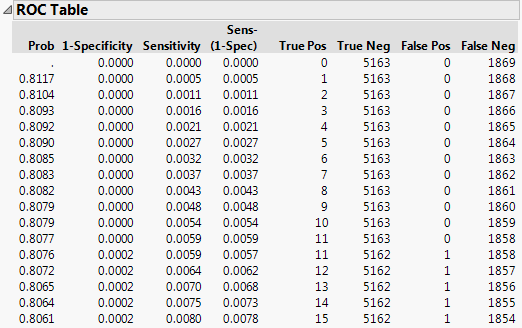
\includegraphics[width=3.0in]{roc_table.png}
\end{figure}

\vspace{-0.3cm}
Here, \texttt{Prob} is what we denoted $p_0$. %\qu{Best model} is not defined here by highest $ACC$ (lowest $ME$), it's determined by highest \textbf{specificity + sensitivity} or equivalently, the highest \textbf{sensitivity - (1 - specificity)}.JMP indicates that row with a $\star$. This is an arbitrary metric, but is a good default.

\end{frame}

\begin{frame}\frametitle{Receiver-Operator Characteristic Curve}

\vspace{-0.2cm}
\begin{figure}
\centering
\hspace{-0.5cm}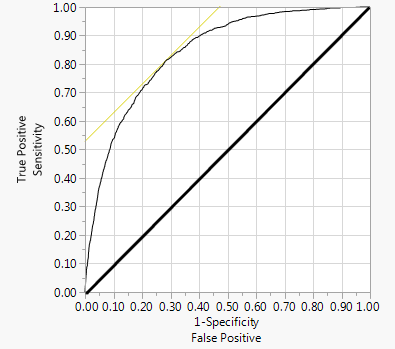
\includegraphics[width=2.4in]{roc_curve.png}
\end{figure}

\small
\vspace{-0.3cm}
The \emph{ROC Curve}. Each dot represents the sensitivity-specificity tradeoff for each $p_0$. The starred row of maximum sensitivity + specificity is indicated here by a yellow tangent line. %\pause I drew the diagonal line to indicate predictive performance that is expected \qu{by chance}. Why? \pause Also, are there other ROC variants? \pause Yes (HW?).

\end{frame}


\begin{frame}\frametitle{Area Under the Curve (AUC) Metric}

\vspace{-0.2cm}
\begin{figure}
\centering
\hspace{-0.5cm}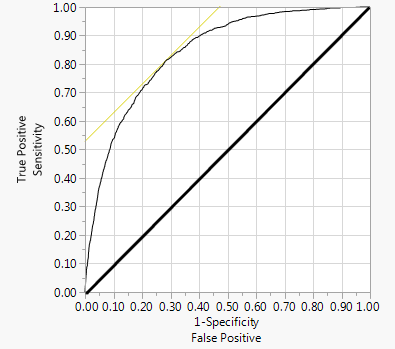
\includegraphics[width=1.3in]{roc_curve.png}
\end{figure}

\small
\vspace{-0.3cm}
If you built a model by chance the \qu{area under the curve} (or to the right of the curve) on the graph would be ...  0.5 since the graph is a unit square. Under the ROC curve itself (or to its right) is an area ...  greater than 0.5. Here, it's 0.844.  This metric is called AUC and is widely used as a metric to assess performance of all possible classifiers in this set of models together, it is a composite metric unlike $ME$ or anything derived from an individual confusion table.\\~\\ 

AUC is nice to evaluate overall performance of all possible models... but at the end of the day...  you ship \emph{ONE} model! So we still need a means of evaluating our one model from one confusion table.

\end{frame}

\begin{frame}\frametitle{Churn Example Where $p_0 = 0.10$}
\pause
\tiny
\begin{table}
\centering
\begin{tabular}{cc|cc|cc}
& $p_0 = 0.5$ & \multicolumn{2}{c|}{$\yhat$} & & Model \\
& & 1 & 0 & Totals &  Errors\\ \hline
\multirow{2}{*}{$y$} & 1 & $TP$ = 1012 & $FN$ = 857 & $P$ = 1869 & $FNR$ = 45.9\% \\ 
& 0 & $FP$ = 531 & $TN$ = 4632 & $N$ = 5163 & $FPR$ = 10.2\% \\ \hline
& Totals & $\Phat$ = 1543 & $\Nhat$ = 5489 & $n=$ 7032 \\
& Use errors & $FDR$ = 34.3\% & $FOR$ = 15.6\% & & \fbox{$ME$ = 19.7\%}
\end{tabular}
\end{table}
\normalsize
\pause

\footnotesize
\begin{table}
\centering
\begin{tabular}{cc|cc|cc}
& $p_0 = 0.1$ & \multicolumn{2}{c|}{$\yhat$} & & Model \\
& & 1 & 0 & Totals &  Errors\\ \hline
\multirow{2}{*}{$y$} & 1 & $TP$ = 1772 & $FN$ = 97 & $P$ = 1869 & $FNR$ = 5.1\% \\ 
& 0 & FP = 2669 & $TN$ = 2494 & $N$ = 5163 & $FPR$ = 51.6\% \\ \hline
& Totals & $\Phat$ = 4441 & $\Nhat$ = 2591 & $n=$ 7032 \\
& Use errors & $FDR$ = 60.1\% & $FOR$ =3.7\% & & \fbox{$ME$ = 39.3\%}
\end{tabular}
\end{table}\pause
\small


Which numbers did not change? \pause $n$, $P$ and $N$. Why? \pause These are fixed according to the dataframe. All other numbers changed! What happend to our first means of evaluation, the Misclassification Error? \pause It increased from 19.7\% $\rightarrow$ 39.3\%. So isn't this a worse model?? \\~\\ \pause 

Not necessarily... It depends on what your goal is!
\end{frame}

\begin{frame}\frametitle{Asymmetric Costs in a Classifier}

These are always two types of errors but the costs are not always the same.

\tiny
\begin{table}
\centering
\begin{tabular}{cc|cc|cc}
& $p_0 = 0.1$ & \multicolumn{2}{c|}{$\yhat$} & & Model \\
& & 1 & 0 & Totals &  Errors\\ \hline
\multirow{2}{*}{$y$} & 1 & $TP$ = 1772 & $FN$ = 97 & $P$ = 1869 & $FNR$ = 5.1\% \\ 
& 0 & FP = 2669 & $TN$ = 2494 & $N$ = 5163 & $FPR$ = 51.6\% \\ \hline
& Totals & $\Phat$ = 4441 & $\Nhat$ = 2591 & $n=$ 7032 \\
& Use errors & $FDR$ = 60.1\% & $FOR$ = 3.7\% & & \fbox{$ME$ = 39.3\%}
\end{tabular}
\end{table}
\small

Imagine we really are the Telecom business manager. It costs 5-10x more to acquire a new customer than to engage a customer who is likely to churn. So you give an incentive package to those who are predicted to churn. \pause Which of the two types of errors specifically is \textit{very} costly? \pause The $FN$. Who are they? \pause These are those who you said were not going to churn \textit{and they did}! Cost? \pause You need to acquire a new customer! The other type of error is less costly, the $FP$. Who are they? \pause These are the people you thought were going to churn and did not. Cost? \pause Whatever the incentive package is.
	
\end{frame}

\begin{frame}\frametitle{Weighted Misclassification Error}

We now define two costs: (1) \pause the cost of the $FP$ denoted $c_{FP}$ and  \pause (2) the cost of the $FN$ denoted $c_{FN}$.  \pause We then define the weighted misclassification error evaluation metric:

\beqn
ME_w := \oneover{n} \sum_{i=1}^n c_{FP} \indic{y_i = 0 \& \yhat = 1} + c_{FN} \indic{y_i = 1 \& \yhat_i = 0}
\eeqn \pause 

We now vary $p_0$ to locate the model that optimizes this error to be minimum.
	
\end{frame}

\begin{frame}\frametitle{Minimum Weighted Misclassification Error}

Let's assume that $c_{FN} = \$1000$ and $c_{FP} = \$100$ just for the example's sake. Note: this is a \emph{cost ratio} of 10:1 (only the ratio matters for the optimal $p_0$ solution).

\vspace{-0.2cm}
\begin{figure}
\centering
\hspace{-0.5cm}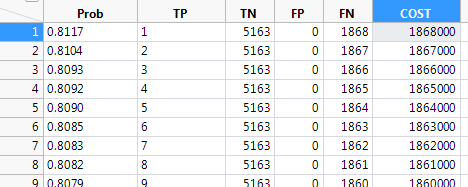
\includegraphics[width=3.1in]{weighted_misclassification_costs.png}
\end{figure}

We now calculate the cost and find the minimum model (i.e. the $p_0$ to ship). [JMP] Beyond scope: some people select the model with the closest $\#FP/\#FN \approx 10:1$ to match the stakeholder preference of the desired cost ratio. I'm not entirely clear on why this fitness function is used. [JMP ratios sheet]



	
\end{frame}

\begin{frame}\frametitle{Expected Value Calculation}

You can also imagine assignment of both costs \textit{and} benefits:

\tiny
\begin{table}
\centering
\begin{tabular}{cc|cc|}
& $p_0 = 0.1$ & \multicolumn{2}{c|}{$\yhat$}   \\
& & 1 & 0  \\ \hline
\multirow{2}{*}{$y$} & 1 & $b_{TP}$ & $c_{FN}$  \\ 
& 0 & $c_{FP}$ &$b_{TN}$  \\ \hline
\end{tabular}
\end{table}\pause
\small

and then use the confusion matrix to estimate probabilities:

\begin{table} \small
\centering
\begin{tabular}{cc|cc|}
& $p_0 = 0.1$ & \multicolumn{2}{c|}{$\yhat$}  \\
& & 1 & 0 \\ \hline
\multirow{2}{*}{$y$} & 1 & 25.1\% & 1.3\%  \\ 
& 0 & 40.0\% & 35.5\%  \\ \hline
\end{tabular}
\end{table}\pause
\small

The expected value would be? 

\beqn
\expe{T} &=& p_{TP} \times b_{TP} +  p_{TN} \times b_{TN} + p_{FP} \times c_{FP} +  p_{FN} \times c_{FN} \\
&\approx& \phat_{TP} \times b_{TP} +  \phat_{TN} \times b_{TN} + \phat_{FP} \times c_{FP} +  \phat_{FN} \times c_{FN}
\eeqn

Highest expected value model is shipped (ex. from Provost \& Fawcett, 2013).
	
\end{frame}

%\begin{frame}\frametitle{$\phat$'s as Ordinal Values}
%
%One final point... If we were on a mission to find the top $m$ churners. What would we do? \pause Sort the $\phat$'s and return the top $m$.
%	
%\end{frame}

\section{Survival Models}

\begin{frame}\frametitle{New Type of Response Metric: TTL}
\small
What if your response was time? For example: \pause

\begin{itemize}
\item Time for a patient to live (typical in clinical trials)? \pause
\item How long will a customer be a customer? \pause
\item How long will a car engine last? \pause
\end{itemize}

What kind of data type is the response? \pause Continuous. \pause But what does response look like at the time of sampling? \\~\\

For example, recall the Telecom churn dataset with one feature (tenure). If the observation has ...

\begin{table}
\centering
\begin{tabular}{ccc}
Tenure Time & Churn? & Total Time as a Customer \\ \hline
2 & Yes & \pause 2 \\
8 & Yes & \pause 8 \\
45 & No & \pause unknown (but known to be $> 45$) \\
\end{tabular}
\end{table}
\normalsize

That third observation's response is \emph{censored}. \pause What are we supposed to do??

\end{frame}

\begin{frame}\frametitle{Dealing with censoring}

One option is to disregard all censored observations. Why is this a bad idea? \pause Selection bias. Our results will only apply to people who have churned. Those people may be different that the general population. \pause Another option is to use \emph{survival modeling}.\\~\\ \pause

This is a very well-studied field with many possible models!
	
\end{frame}

\begin{frame}\frametitle{The Exponential Model}
\small
Assume $Y$ now is time. Time must be positive!

\beqn
Y = f(x_1, \ldots, x_p) + \errorrv
\eeqn

We have to be careful to make $f$ positive and $\errorrv$ negative but not too negative to make $Y < 0$. \pause One such model is the exponential model with conditional mean $f(x_1, \ldots, x_p)$.

\beqn
Y \sim Exp(f(x_1, \ldots, x_p))
\eeqn

Let's review the exponential r.v. \pause If $Y \sim Exp(\mu)$, then its density function and cumulative density functions are

\beqn
p(y) = \oneover{\mu} e^{-\oneover{\mu} y} \quad \text{and} \quad F(y) = 1 - e^{-\oneover{\mu} y}
\eeqn

with mean $\expe{Y} = \mu$ where $\mu > 0$. \pause So if $Y \sim Exp(17)$, you expect the observation to be ... \pause 17 on average.

\end{frame}

\begin{frame}\frametitle{The Exponential Log-Linear Model (ELLM)}

Let's say we want to use our linear model $\beta_0 + \beta_1 x_1 + \ldots + \beta_p x_p$ for the conditional mean. Problem? \pause Yes. The mean can only be a number greater than zero. Hence we need the $\lambda$ link function again! How can we convert $s_\reals = \beta_0 + \beta_1 x_1 + \ldots + \beta_p x_p$ to something between $0$ and $+\infty$? \pause Without going into many different link function, let's just use the natural exponential:

\beqn
s = \lambda(s_\reals) = \pause e^{s_\reals} \quad \Rightarrow \quad \pause s = e^{\beta_0 + \beta_1 x_1 + \ldots + \beta_p x_p} \pause
\eeqn

And voila we have our survival model:

\beqn
Y \sim Exp(e^{\beta_0 + \beta_1 x_1 + \ldots + \beta_p x_p})
\eeqn

Interpretation of a unit change in $x_1$? \pause With all other variables kept constant, a unit change in $x_1$ will multiply the expected survival by $e^{\beta_1}$ in a naturally observed new object.
	
\end{frame}

\begin{frame}\frametitle{Assumptions of an ELLM}

Next up in the recipe... we need to get estimates of the true parameters, we have been denoting these $\braces{\betahat_0, \betahat_1,  \ldots, \betahat_p}$. How to do so? \pause Maximum Likelihood (just like linear regression and logistic regression). We will first need the \qu{ELLM assumptions}


\begin{enumerate}
\item Independence among observations. Thus,\pause 

\footnotesize
\beqn
&&\cprob{Y_1 = y_1, Y_2 = y_2, \ldots, Y_n = y_n}{\X_1 = \x_1, \X_2 = \x_2, \ldots, \X_n = \x_n} \\
&=& \prod_{i=1}^n \cprob{Y_i = y_i}{\X_1 = \x_i}
\eeqn

\small
\item Exponential Model. Thus, \pause
\footnotesize
\beqn
= \prod_{i=1}^n \oneover{\mu} e^{-\oneover{\mu} y_i}
\eeqn \pause
\small
\item Log-Linear conditional expectation. Thus,


\end{enumerate}

\end{frame}

\begin{frame}\frametitle{Fitting an ELLM}
\footnotesize
\beqn
= \prod_{i=1}^n \oneover{e^{\beta_0 + \beta_1 x_{i1} + \ldots + \beta_p x_{ip}}} e^{-\oneover{e^{\beta_0 + \beta_1 x_{i1} + \ldots + \beta_p x_{ip}}} y_i}
\eeqn \pause
Can we just maximize the above over all values of the $\beta$'s like before? \pause We are missing one thing. What if survival time is a censored value (denoted $y_i'$)? All we know about that $y_i$ is that it's greater than the last value recorded! \pause Recall $\prob{Y > y} = 1 - F(y) = e^{-\oneover{\mu} y}$\\~\\

Let $c_i$ indicate censorship: 1 if censored and 0 if not. Our likelihood is now in two pieces:

\beqn
&=& \prod_{i=1}^n \tothepow{\oneover{e^{\beta_0 + \beta_1 x_{i1} + \ldots + \beta_p x_{ip}}} e^{-\oneover{e^{\beta_0 + \beta_1 x_{i1} + \ldots + \beta_p x_{ip}}} y_i}}{1 - c_i} \pause \prob{Y > y_i'}^{c_i} \pause \\
&=& \prod_{i=1}^n \tothepow{\oneover{e^{\beta_0 + \beta_1 x_{i1} + \ldots + \beta_p x_{ip}}} e^{-\oneover{e^{\beta_0 + \beta_1 x_{i1} + \ldots + \beta_p x_{ip}}} y_i}}{1 - c_i} \tothepow{e^{-\oneover{\beta_0 + \beta_1 x_{i1} + \ldots + \beta_p x_{ip}} y_i'}}{c_i} \pause
\eeqn 
	
Now the computer crunches away (similar to a logistic regression fit) and we get values of $\braces{\betahat_0, \betahat_1,  \ldots, \betahat_p}$ back in a split second. \pause Now for inference...
\end{frame}

\begin{frame}\frametitle{Global Test in Survival ELLM Regression}

\footnotesize
Just like in logistic regression, we can make use of the ... \pause likelihood ratio test. \pause Recall:

\vspace{-0.2cm}
\beqn
LR :=
%
\displaystyle \max_{\theta \in \Theta} \lik{\theta; x}
%
/
%
\displaystyle \max_{\theta \in \Theta_R}  \lik{\theta; x}
%
\eeqn

Let's now do a \qu{whole model} / \qu{global} / \qu{omnibus} test: \pause

\beqn
&& H_0: \beta_1 = 0, \beta_2 = 0, \ldots, \beta_p = 0, \quad H_a: \text{at least one is non-zero}
\eeqn

So $\Theta$ would be the space of all $\beta_0, \beta_1, \ldots, \beta_p$ and $\Theta_R$ will restrict the space to only $\beta_0$ with zeroes for all other \qu{slope} parameters.

\tiny
\beqn
LR = \frac{
\displaystyle \max_{\beta_0, \beta_1, \ldots, \beta_p} 
\lik{\beta_0, \beta_1, \ldots, \beta_p; y_1, \ldots, y_n, c_1, \ldots, c_n, \x_1, \ldots, \x_n}
}{
\displaystyle \max_{\beta_0} 
\lik{\beta_0, \beta_1 = 0, \ldots, \beta_p = 0; y_1, \ldots, y_n, y_n, c_1, \ldots, c_n,  \x_1, \ldots, \x_n}
}
\eeqn \pause

\small
So in the numerator the computer iterates to find $\braces{\betahat_0, \betahat_1,  \ldots, \betahat_p}$, plugs it in and computes the likelihood and in the denominator the computer independently iterates to find $\braces{\betahat_0}$, plugs it in and computes the likelihood, then together, the $LR$.
\end{frame}

\begin{frame}\frametitle{Partial Tests in Survival Regression}

\small
We then look at $Q = 2\natlog{LR}$ and compare it to the appropriate $\chi^2$ distribution. Here, since we've dropped $p$ parameters / degrees of freedom, we look at the critical $\chisq{p, \alpha}$ value.\\~\\ \pause

Let's say we want to test something like:

\beqn
&& H_0: \beta_1 = 0 ~\&~ \beta_2 = 0, \quad H_a: \text{at least one is non-zero}
\eeqn

We can again use the likelihood ratio test:

\tiny
\beqn
LR = \frac{
\displaystyle \max_{\beta_0, \beta_1, \ldots, \beta_p} 
\lik{\beta_0, \beta_1, \ldots, \beta_p; y_1, \ldots, y_n, c_1, \ldots, c_n, \x_1, \ldots, \x_n}
}{
\displaystyle \max_{\beta_0, \beta_3, \ldots, \beta_p} 
\lik{\beta_0, \beta_1 = 0, \beta_2 = 0, \beta_3, \ldots, \beta_p = 0; y_1, \ldots, y_n, c_1, \ldots, c_n, \x_1, \ldots, \x_n}
}
\eeqn \pause
\small
We then look at $Q = 2\natlog{LR}$ and compare it to the appropriate $\chi^2$ distribution. Here, since we've dropped $2$ parameters / degrees of freedom, we look at the critical $\chisq{2, \alpha}$ value.

\end{frame}

\begin{frame}\frametitle{Individual Tests in Survival Regression}

Let's say we want to test an individual slope coefficient:

\beqn
&& H_0: \beta_j = 0, \quad H_a: \beta_j \neq 0
\eeqn
	
(a la the \qu{partial-F test}). We can again use the likelihood ratio test:

\tiny
\beqn
\hspace{-10pt} LR = \frac{
\displaystyle \max_{\beta_0, \beta_1, \ldots, \beta_p} 
\lik{\beta_0, \beta_1, \ldots, \beta_p; y_1, \ldots, y_n, c_1, \ldots, c_n, \x_1, \ldots, \x_n}
}{
\displaystyle \max_{\beta_0, \beta_1, \ldots, \beta_{j-1}, \beta_{j+1}, \ldots \beta_p} 
\lik{\beta_0, \beta_1, \ldots, \beta_{j-1}, \beta_j = 0, \beta_{j+1}, \ldots \beta_p; y_1, \ldots, y_n, c_1, \ldots, c_n, \x_1, \ldots, \x_n}
}
\eeqn \pause

\small
We then look at $Q = 2\natlog{LR}$ and compare it to the appropriate $\chi^2$ distribution. Here, since we've dropped 1 parameter / degrees of freedom; thus we look at the critical $\chisq{1, \alpha}$ value. \\~\\ \pause

And again: a $\chisq{}$ r.v. with one degree of freedom has the following cool property: $Q \sim \chisq{1} \Rightarrow \pause \sqrt{Q} \sim \stdnormnot$ i.e. a \qu{z-score}. This is how JMP produces standard errors for survival regression coefficients.

\end{frame}

\begin{frame}\frametitle{Simple Survival Regression and Predictions}
\small
How do we predict?

\vspace{-0.2cm}
\beqn
\yhat= \yhat(\x^*) = \pause e^{\betahat_0 + \betahat_1 x_1^* +  \ldots + \betahat_p x_p^*}
\eeqn

What are we predicting? \pause Average time to survive. \\~\\
\vspace{-0.2cm}
Let's return to the Telecom example and look at just \qu{\texttt{SeniorCitizen}} on customer lifetime. [JMP] \pause Is this variable significant? \pause Yes. \pause Now let's predict the time for a new non-senior citizen:

\beqn
\yhat = \yhat(\x^*) = \pause e^{\betahat_0 + \betahat_1 (0)} = \pause e^{4.915} = 136.6
\eeqn

Now let's predict the time for a new senior citizen: \pause

\beqn
\yhat = \yhat(\x^*) = \pause e^{\betahat_0 + \betahat_1 (1)} = \pause e^{4.915 + -0.535} = 79.84
\eeqn

 Is the reduction expected? \pause Yes. Why are these numbers so large? \pause (1) Likely the exponential model is not a great fit here since the tail is too long and the memorylessness property is not realistic. Also, \pause (2) Dataset is not a good sample... was not \emph{designed} for survival.
	
\end{frame}

\begin{frame}\frametitle{Multivariable Survival Regression}

[JMP] 
\begin{itemize}
\item Do these coefficients make sense? \pause 
\item What's wrong with this dataset?? \pause The max survival is 72mo and there's thousands of cases that are censored. \pause
\item Evaluating the fitness (i.e. $R^2, RMSE, ME_w$, etc) of survival models is complicated... not covered.
\end{itemize}	
\end{frame}

\section{Non-linearity \& Interactions}

\begin{frame}\frametitle{Simple Test of Linearity}

Here's the \qu{Medicorp} dataset. The response is sales (in \$1000's) and the features are advertising (in \$1000's), American region and bonus for the sales team (in \$1000's). \\~\\ \pause

Let's look at a simple regression of sales on bonus. \pause Are we sure this is linear? Or are there diminishing returns? How to test diminishing returns? \pause Quadratic fit is one way. We should see what kind of sign on the squared term? \pause Negative. And we do. And it's pretty significant... could you make a case of dredging here? \pause Probably not. Are we sure it's quadratic diminishing returns? \pause Nope... that's much harder to test... beyond scope of course... and probably not all that interesting. \pause What's the takeaway message here? \pause You should give bonuses but don't make them \qu{too} big. \\~\\

\small
Interpretation of unit change in $x:$ bonus? Depends on the value where you start from (we are moving away from simple interpretations).
	
\end{frame}


\begin{frame}\frametitle{Polynomial Regression}

Let's try to fit a better curve to bonus --- a 4-degree polynomial. Seems to fit better than a quadratic [see LRT in R]. What's the interpretation of a 4-degree polynomial model?? \pause Not so intuitive unfortunately. Rarely do we see parametric pre-designed models with more than a quadratic term.

\end{frame}

\begin{frame}\frametitle{Continuous : Categorical Interactions}

It's possible that bonuses may have differential effects in the different American \qu{regions}. The way to test this is to allow for a differential slope for each region. [JMP] \pause


\begin{figure}
\centering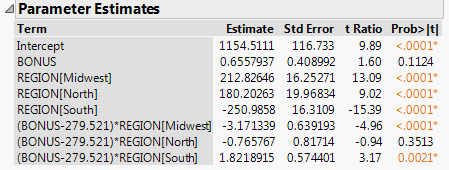
\includegraphics[width=3in]{interactions.png}
\end{figure}

How can we interpret this? \pause Could we also interact two continuous features? Two categorical features? Could we interact features with others' polynomials? Yes, yes, yes...
	
\end{frame}

\begin{frame}\frametitle{Theories versus Prediction}

Above we tested the predictive power of non-linearities in two ways \pause (1) creating polynomial extensions to given features and finding curvilinear patterns and \pause (2) creating differential slopes based of one variable when isolating based on the value of another variable. \\~\\

However, we had specific theories to test in mind \pause (1) diminishing returns and (2) effects of incentivizing bonuses in different parts of the country. \\~\\

What if we had no theories to test, but we wanted to fit the data as best as possible (i.e. non-parametric)? \pause Try everything... all polynomial terms up to 5, all interactions with up to the squared terms. [JMP medicorp\_exp] \pause We got $R^2 = 98\%$ which rocks!! But none of our variables are significant.... why? \pause Massive collinearity all over the place! do we give a hoot if we only care about predictive accuracy? \pause NO. \pause But... is the $R^2 = 98\%$ real? \pause NO...
	
\end{frame}

\section{Overfitting}

\begin{frame}\frametitle{The First Clue of Trouble in Paradise...}
\pause
was that F-test demo from Lecture 2 where

\beqn
x &=& \braces{0, 0.1, 0.2, \ldots, 10.0} \\
Y &\sim& x + \errorrv \\
\errorrv &\sim& \normnot{0}{5^2}
\eeqn

 [repeat in R]. \pause Here, the $R^2$ goes from 22\% up to 

\begin{itemize}
\item 99.5\% all on completely random data which you know is fake!! \pause
\item 99.9\% on splines (polynomials on steroids) which may not be fake??
\end{itemize}

How do we know?
	
\end{frame}

\begin{frame}\frametitle{Recall the Modeling Basics}

In lecture 1 we spoke about how

\beqn
Y = f(x_1, \ldots, x_p) + \errorrv
\eeqn

where $x_1, \ldots, x_p$ denotes \pause predictors available (including all polynomials and interactions and whatnot!) and $\errorrv$ denotes \pause \emph{irreducible error} due to information not available (and thus independent of $x_1, \ldots, x_p$), the inaccessible information. \\~\\ \pause

By including all sorts of polynomials and interactions, we become more nonparametric thereby losing the benefits of the parametric worldview of $s$... \pause (i.e. parsimony, \pause interpretability \pause and inference) but gaining a closer fit of the true $f$. But what could go wrong if we take this liberty? \\~\\
	
\tiny
Non-germane footnote: recall that we fit $\hat{s}$ which generally speaking fails to estimate $s$ correctly (model error) and $s$ generally speaking fails to represent $f$ correctly since its a parametric model which lacks flexibility. \\~\\ \pause
\end{frame}

\begin{frame}\frametitle{Going Too Far}

\beqn
Y = f(x_1, \ldots, x_p) + \errorrv
\eeqn

It's possible our $\hat{f}$ can estimate $f$ (which is good) but... \pause it can encroach on and start fitting and optimizing the $\errorrv$. Why is this bad? \pause Since $\errorrv$ is independent of $x_1, \ldots, x_p$, it is creating a random fit. \pause Random fits are akin to \qu{making up a model} and it is the opposite of the \qu{data-driven approach}. \\~\\ \pause

Any value different from $f$ is not \emph{generalizable} as the conditional mean minimizes squared error. \\~\\ \pause

But the BIG problem is: we don't know what the form of $f$ is and we don't know the individual values of $\errorrv$. Thus, we have NO WAY to know if we've overfit (as of now)!
	
\end{frame}

\begin{frame}\frametitle{When Does This Happen?}
\footnotesize
Essentially, when $p$ gets closer to $n$. Here's the linear model case with $n=2$ and there's one slope so $p=1$ (+1 for the intercept) so really, the number of predictors is 2 since there is two degrees of freedom. [R demo]

\vspace{-0.3cm}
\begin{figure}
\centering
\hspace{-0.5cm}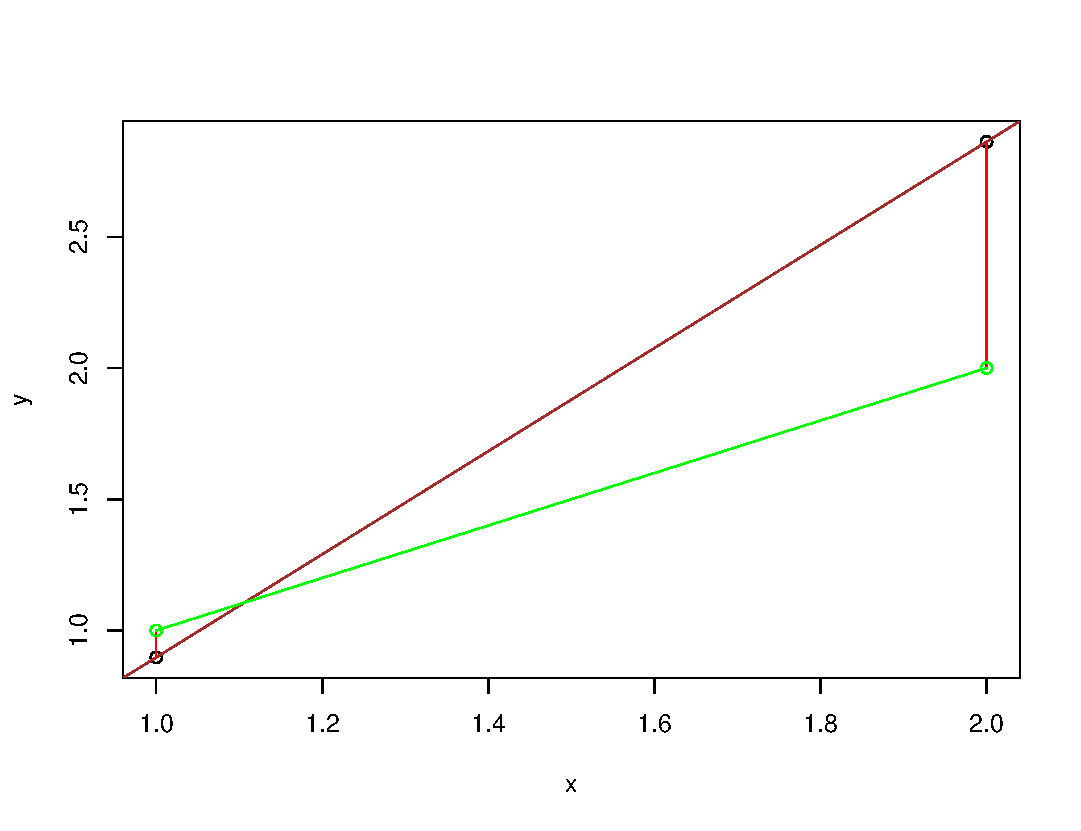
\includegraphics[width=2.0in]{overfitting_simple}
\end{figure}
\vspace{-0.5cm}
\footnotesize
The green is the true conditional expectation function $f(x)$ and the brown is the fitted model and the red are the true $\errorrv_1$ and $\errorrv_2$ values. Where are $e_1$ and $e_2$? \pause They are zero (and thus not pictured). The fitted model has $R^2 = 100\%$. Recall from middle school... when they asked you to draw a line between two points --- the line perfectly goes through two points. \pause Why are the $\se{\betahat_j}$'s \texttt{NA}? \pause Division by zero. \pause Can you imagine two predictors and three points and a plane? \pause What about in a logistic regression? [Whiteboard demo]
	
\end{frame}

\begin{frame}\frametitle{Assessing Overfitting and its Cost to You}
\small
Overfitting comes from over-optimizing a sample (i.e. fitting $\errorrv$) and thus having poor generalizability and thus poor predictive performance in the future! \\~\\ \pause

Let's return to the [R demo] to witness the cost of overfitting. \pause How did we demonstrate overfittedness? \pause We used \qu{new data} not in the dataframe generated from the same realization process as the historical dataframe (our sample). Hence this new data is called \emph{out of sample (oos)} data. And then we calculated familiar metrics such as SSE, RMSE, $R^2$ but since these are done oos, we call them oosSSE, oosRMSE, oos$R^2$ and they are our \emph{out of sample statistics}. Everything we spoke about previously we will now call \emph{in-sample statistics}.

\begin{table}
\centering
\begin{tabular}{rcc}
& In Sample & Out of Sample \\ \hline
RMSE   & 2.0 & 84.7 \\
$R^2$ & 99.9\% & 9.5\%
\end{tabular}
\end{table}

Overfitting can get arbitrarily bad and this is an extreme example.
	
\end{frame}

\section{Model Validation}

\begin{frame}\frametitle{Assessments in the Real World}
\small
It is easy to assess if you have access to the data-generating process --- you can just generate more data and see how you do. But in the real world, you only have a limited set of historical data from the data-generating process. What to do?\\~\\ \pause

Why not \textit{imagine} some of your historical data is future data. That is, split your dataframe into two pieces: \pause

\begin{enumerate}
\item What we've been calling the historical dataframe but now will calling the \qu{training set}. We use this to build the model, as we've done. \pause
\item The \qu{test set} that is the piece you are imagining to come in the future. his gives you a means to evaluate your model you built from the training set. \pause
\end{enumerate}

Building the model on the training set and predicting on the test set and comparing these predictions to the real, known values of the response in the test set constitutes \textit{out of sample validation}. Why is it called that?

\end{frame}

\begin{frame}\frametitle{Model Fitting with OOS Validation}

\begin{figure}
\centering
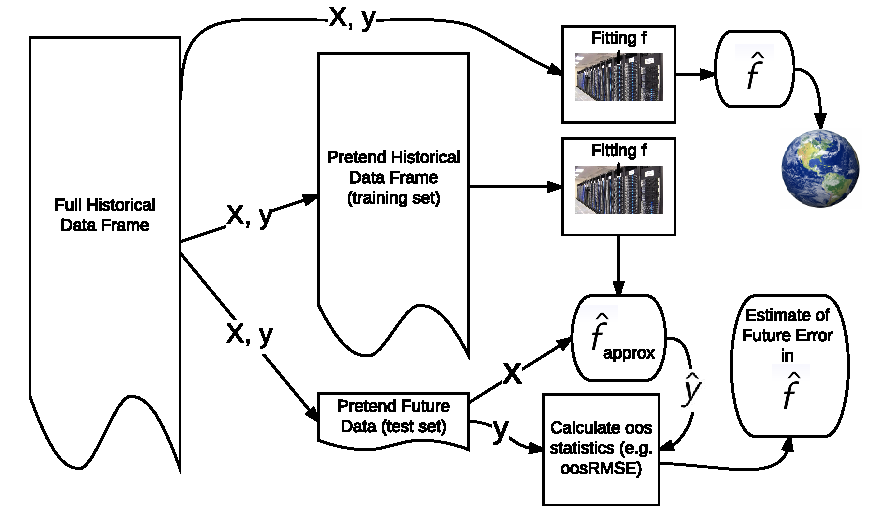
\includegraphics[width=4.1in]{oos_validation}
\end{figure}

Can oos metrics be better than in-sample metrics (on average)? \pause No...
\end{frame}

\begin{frame}\frametitle{A Possible Spin on Validation}
\footnotesize
Procedure outlined above:
	
\begin{enumerate}\footnotesize
\item Split dataframe into training and test. \pause
\item Build model on training. \pause
\item Predict using the test set. \pause 
\item Calculate estimate of future generalization error.
\end{enumerate}


Does the following procedure also seem reasonable?
	
\begin{enumerate}\footnotesize
\item Split dataframe into training and test.
\item Build model A on training.
\item Predict using the test set. 
\item Calculate estimate of future generalization error of model A. \pause
\item Build a different model B on training. \pause
\item Predict using the test set.  \pause
\item Calculate estimate of future generalization error of model B. \pause
\item Pick whichever model has better generalization error.
\end{enumerate}

\end{frame}

\begin{frame}\frametitle{Valid Validation}

What's wrong? \pause You snooped the test set... \pause analagous to looking into the future and \pause seeing results and saying \qu{I don't like em}, \pause then returning to the past and trying again. \pause This can lead to very optimistic results --- it is essentially overfitting and you've tricked yourself into thinking you are honest. \\~\\

\pause The oos validation is only valid if...

\begin{figure}
\centering
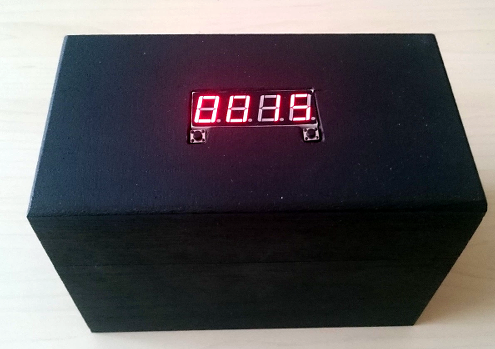
\includegraphics[width=1.2in]{lockbox.png}
\end{figure}

you treat the test set as a lockbox. Once you open it up, that's it!
	
\end{frame}

\begin{frame}\frametitle{Training-Test Splitting}
\footnotesize
We have a choice to split our dataframe into two pieces. Assuming each data point is independent (the running assumption), you should do this completely randomly. When would this assumption not be true? \pause For example, a time series.\\~\\ \pause
\vspace{-0.2cm}

How large should the test set be? Usual sizes are 10-30\%. What's the tradeoff? If the test set is larger, then ...\pause
 
\begin{enumerate}\footnotesize
\item the more accurate the assessment of generalization error would be (less variance) and \pause
\item the less accurate the model will be since it's fitting with less data (more bias) \pause
\end{enumerate}

If the test set is smaller then vice versa:

\begin{enumerate}\footnotesize
\item the less accurate the assessment of generalization error would be (more variance) and \pause
\item the more accurate the model will be since it's fitting with less data (less bias) \pause
\end{enumerate}

Note: the in-sample and oos statistics are statistics! Thus, they are random!

\end{frame}

\begin{frame}\frametitle{Doing oos Validation in JMP}

Let's take a look at the medicorp data and validate it. Recall, the in-sample $R^2 \approx 98\%$ and the in-sample RMSE is about 48.9. \pause \\~\\

[JMP Cols...Modeling Utilities...Make Validation Col...fit model... validation option is the validation col...crossvalidation tab] Note: \qu{RASE} = root average squared error = root mean squared error = oosRMSE. \qu{Validation} = \qu{test}. \qu{Freq} is the sample sizes in training and test. Looks like we were overoptimistic by 6x the standard error on predictions! Substantial overfitting.

\end{frame}

\begin{frame}\frametitle{Validating Multiple Models}

Let's look at three models for the White Wine data. Here the response is wine quality as measured by professional raters and features are 11 features (e.g. acidity, sugar, pH and alcohol content).

\begin{enumerate}
\item[A] plain linear model \pause
\item[B] six-degree polynomials for all features \pause
\item[C] six-degree polynomials and all first-order interactions \pause
\item[D] six-degree polynomials and all interactions up to 11th order \pause
\end{enumerate}

[JMP col validation... fit all models with validation ... save prediction formula cols... analyze model... model comparison] Conclusions? \pause Model C looks the best. Where to go from here?\\~\\

What did I do that wasn't legal? Remember a few slides ago? I looked at the test set four times! We need to solve this problem...
	
\end{frame}




\end{document}
	



\begin{frame}\frametitle{}

	
\end{frame}

\begin{frame}\frametitle{}

	
\end{frame}






\begin{frame}\frametitle{}

	
\end{frame}



\begin{frame}\frametitle{}

	
\end{frame}

\begin{frame}\frametitle{}

	
\end{frame}


\begin{frame}\frametitle{}

	
\end{frame}

\begin{frame}\frametitle{}

	
\end{frame}


\begin{frame}\frametitle{}

	
\end{frame}

\begin{frame}\frametitle{}

	
\end{frame}


\begin{frame}\frametitle{}

	
\end{frame}

\begin{frame}\frametitle{}

	
\end{frame}


\begin{frame}\frametitle{}

	
\end{frame}

\begin{frame}\frametitle{}

	
\end{frame}


\begin{frame}\frametitle{}

	
\end{frame}

\begin{frame}\frametitle{}

	
\end{frame}


\begin{frame}\frametitle{}

	
\end{frame}

\begin{frame}\frametitle{}

	
\end{frame}


\begin{frame}\frametitle{}

	
\end{frame}

\begin{frame}\frametitle{}

	
\end{frame}


\begin{frame}\frametitle{}

	
\end{frame}

\begin{frame}\frametitle{}

	
\end{frame}